\chapter{Materiales y métodos} 

% ------------------------------------------------------------------------------------------------------------
% ------------------------------------------------------------------------------------------------------------

\section{Conjunto de datos disponibles}

Disponemos de un conjunto de datos compuesto por radiografías panorámicas maxilofaciales de individuos de 12 países distintos (véase en la Tabla \ref{tab:instituciones_fuente_dataset}), obtenidas con distintos modelos de máquinas de rayos X%
\footnote{
    Los modelos empleados fueron: \textit{Planmeca Promax Digital Panoramic}; \textit{Sirona ORTHOPHOS-XG}, \textit{ORTHOPHOS-DS}, y \textit{SIDEXIS}. Las constantes radiológicas usadas fueron de 66 a a 70 kV, 7 a 11 mA, y 15 s.
}.
Este conjunto de datos ha sido sido proporcionado por Panacea Cooperative Research, empresa \textit{spin-off} de la Universidad de Granada. El \textit{dataset} incluye:


\begin{table}[h]
    \small
    \centering
    \begin{tabular}{@{}clc@{}}
    \toprule
    PAÍS                                                            & INSTITUCIONES                                                                                                                                                            & Nº DE EJEMPLOS \\ \midrule
    \begin{tabular}[c]{@{}c@{}}Bosnia y \\ Herzegovina\end{tabular} & Universidad de Sarajevo                                                                                                                                                  & 882            \\ \hline
    Botsuana                                                        & \begin{tabular}[c]{@{}l@{}}Dos clínicas dentales privadas en \\ Garobone\end{tabular}                                                                                    & 1242           \\ \hline
    Chile                                                           & \begin{tabular}[c]{@{}l@{}}Dos clínicas dentales privadas en \\ Santiago y Rancagua\end{tabular}                                                                         & 1016           \\ \hline
    \begin{tabular}[c]{@{}c@{}}República \\ Dominicana\end{tabular} & \begin{tabular}[c]{@{}l@{}}Tres clínicas dentales privadas en \\ Santo Domingo, La Vega y Santiago\end{tabular}                                                          & 541            \\ \hline
    Japón                                                           & \begin{tabular}[c]{@{}l@{}}Department of Forensic Sciences, \\ Iwate Medical University, Iwate\end{tabular}                                                              & 1045           \\ \hline
    Corea del Sur                                                   & Catholic University of Korea, Seoul                                                                                                                                      & 500            \\ \hline
    Malasia                                                         & \begin{tabular}[c]{@{}l@{}}Faculty of Dentistry Universiti Teknologi \\ MARA Selangor Branch, Selangor\end{tabular}                                                      & 667            \\ \hline
    Turquía                                                         & \begin{tabular}[c]{@{}l@{}}Department of Dentomaxillofacial \\ Radiology, Baskent University, Turkey\end{tabular}                                                        & 2323           \\ \hline
    Uganda                                                          & \begin{tabular}[c]{@{}l@{}}Department of Dental Morphology with \\ the Université Claude Bernard Lyon 1, \\Faculté d’odontologie, Lyon\end{tabular}                      & 283            \\ \hline
    Italia                                                          & \begin{tabular}[c]{@{}l@{}}Department of Surgical Sciences, \\ University of Cagliari\end{tabular}                                                                       & 173            \\ \hline
    Kosovo                                                          & \begin{tabular}[c]{@{}l@{}}University Dentistry Clinical Center, \\ Pristina\end{tabular}                                                                                & 1397           \\ \hline
    Líbano                                                          & Clínica dental privada en Beirut                                                                                                                                         & 690            \\ \bottomrule
    \end{tabular}
    \caption[
        Lista de instituciones participantes en la recolección de los datos e imágenes dentales utilizados en el trabajo.
    ]{   
        Lista de instituciones participantes en la recolección de los datos e imágenes dentales utilizados en el trabajo.
    }
    \label{tab:instituciones_fuente_dataset}
\end{table}

\begin{itemize}

    \item datos tabulares (en formato CSV), donde cada fila representa un ejemplo (un individuo), con los siguientes campos: un identificador único, sexo del individuo, edad del individuo y ``sample'' (clasificación según el origen geográfico de la radiografía).

    \item imágenes bidimensionales de radiografías panorámicas maxilofaciales, con una imagen asociada a cada individuo mediante su ID único. 

\end{itemize}

Se proporcionan los datos ya preprocesados, por lo que no es necesario realizar tareas adicionales de limpieza o transformación previa antes de su análisis. Se ha ignorado el campo ``sample'', dado que se trata de una asignación sesgada y no representa necesariamente una clasificación fiable del origen poblacional de los individuos. Por tanto, este campo no se emplea en el análisis ni en el entrenamiento de los modelos, centrándose exclusivamente en las variables de edad, sexo e imagen.

Hay un total de 10 739 ejemplos, de los que 5756 son de individuos de sexo femenino y 4983 de sexo masculino. Las edades mínima y máxima son 14 y 26 años, respectivamente, y la media son 19.13 años. 
En la Figura \ref{fig:histogram_ages_sex} se observa que el número de ejemplos por edad se mantiene relativamente constante desde los 14 hasta los 21 años, a partir de los cuales disminuye progresivamente, con una representación notablemente menor en los grupos de 24, 25 y 26 años.
En esta figura también podemos comprobar la distribución de ejemplos en cada edad por sexo, y observamos que hay ligeramente más ejemplos del sexo femenino que del masculino para prácticamente todas las edades.

\begin{figure}[H]
    \centering
    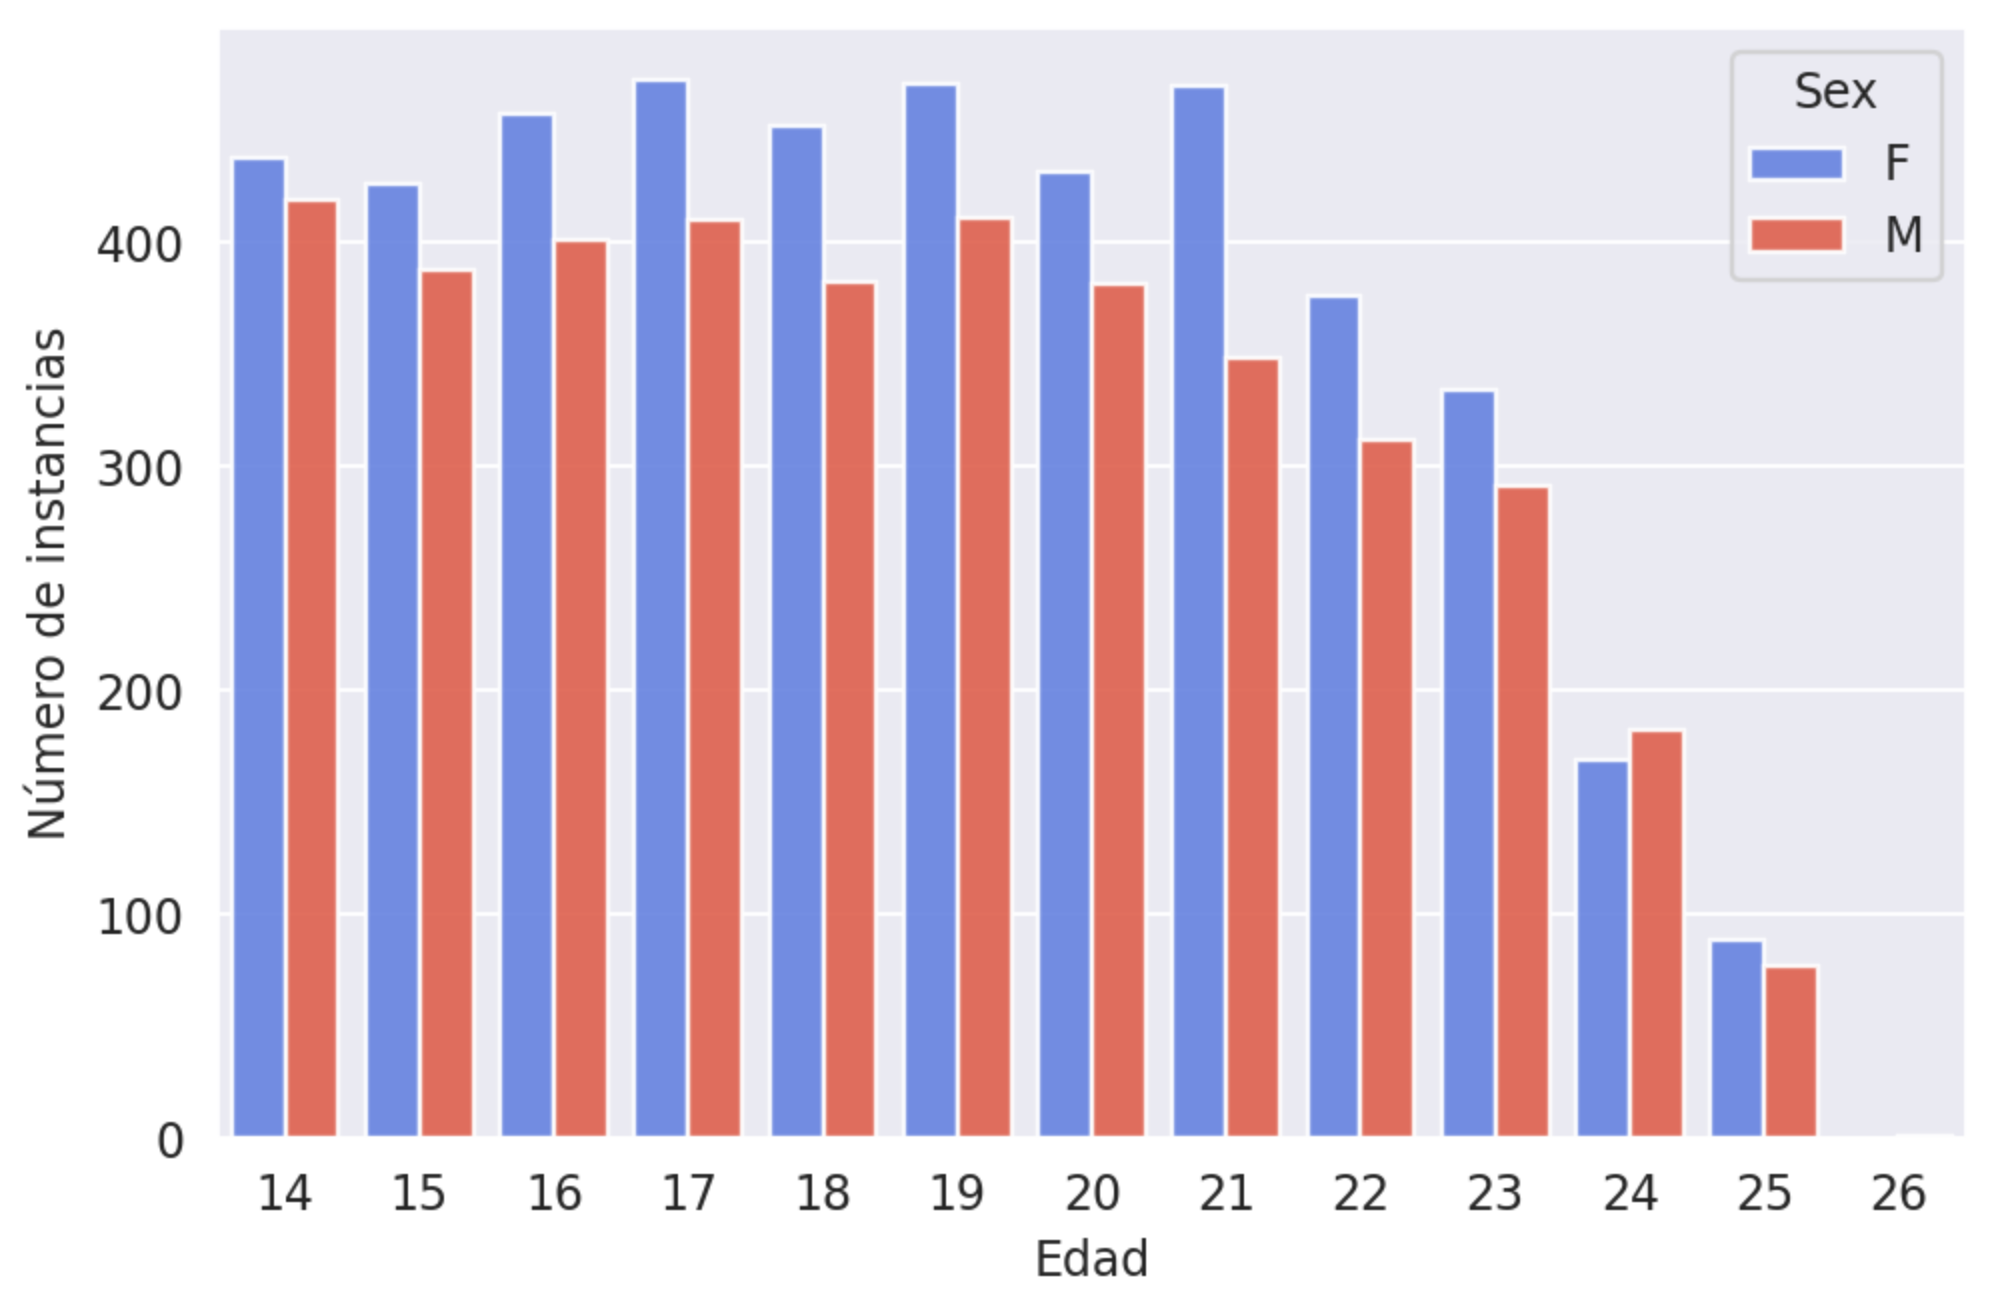
\includegraphics[width=0.7\textwidth]{capitulos/cap_04/imagenes/histogram_by_age_and_sex.png}
    \caption[
        Histograma de edades de los individuos del conjunto de datos disponible diferenciado por sexo.
    ]{
        Histograma de edades de los individuos del conjunto de datos disponible diferenciado por sexo. 
    } 
    \label{fig:histogram_ages_sex}
\end{figure}

En conclusión, el dataset no presenta desbalances extremos, lo que permite un análisis representativo de la población incluida. No obstante, será necesario examinar con mayor detalle la infrarrepresentación de la población de mayor edad, especialmente a partir de los 22 años, para evaluar su posible impacto en el rendimiento y generalización de los modelos entrenados

Se proporcionan los datos ya divididos en \textit{train} ---con un 80\% de los individuos--- y \textit{test} ---con el 20\% restante---, con la intención de que puedan ser utilizados para entrenar y evaluar modelos de predicción. La división de ambos conjuntos se hizo de forma estratificada, de lo que se asume que la distribución será igual en ambos datasets. 

\FloatBarrier

% ------------------------------------------------------------------------------------------------------------
% ------------------------------------------------------------------------------------------------------------


\section{Métodos propuestos}

\subsection{Arquitectura empleada}

Se avanza que los problemas planteados en el siguiente capítulo parten de imágenes bidimensionales de las radiografías panorámicas maxilofaciales como entrada, y estimación de edad o sexo a la salida.

Como modelo, se ha decidido emplear una CNN, dado su buen desempeño en tareas de visión por computador. Específicamente, se ha optado por la arquitectura ResNeXt50 \cite{xie2017} preentrenada en Imagenet \cite{deng2009} como punto de partida. Aunque ResNeXt50 fue entrenado originalmente para una tarea de clasificación, se puede adaptar fácilmente a tareas de regresión ---como la estimación de edad--- reemplazando su capa final por una capa de salida adecuada. Por otro lado, a pesar de haber sido entrenado en un dominio diferente al de nuestro problema, el uso de pesos preentrenados ofrece una ventaja significativa: permite una inicialización más robusta que comenzar desde cero, ya que la arquitectura ya ha aprendido a extraer patrones visuales básicos, como bordes y texturas, mediante filtros genéricos.

% ------------------------------------------------------------------------------------------------------------

\subsection{Regresión cuantílica}

La \textbf{regresión cuantílica (\textit{quantile regression}, \acrshort{QR})} es un tipo de regresión que, a diferencia de la regresión puntual, predice intervalos o cuantiles específicos de la distribución de la variable respuesta, en lugar de solo su media. Esta técnica parte de la noción de que la inferencia estadística no se limita a un valor único, sino que puede representarse mediante una distribución de valores probables, de la cual es posible estimar ciertos cuantiles para describir la variabilidad del comportamiento de la variable objetivo.

En este sentido, la regresión cuantílica permite modelar límites inferiores y superiores (por ejemplo, el percentil 10\% y 90\%) para capturar la incertidumbre o heterocedasticidad en los datos. No debe confundirse con una técnica de \acrshort{UQ}, ya que no modela explícitamente la incertidumbre epistémica ni proporciona garantías estadísticas de cobertura como lo hacen los métodos de predicción conformal. Sin embargo, puede utilizarse como parte de un enfoque para cuantificar la incertidumbre aleatoria o condicional al estimar intervalos de predicción directamente a partir de los datos.

Esta técnica de regresión puede implementarse solo en arquitectura de redes neuronales y modelos tipo \textit{ensemble}, aunque su implementación difiere significativamente. 

En redes neuronales, esta regresión requiere de:

\begin{itemize}

    \item Definir una capa de salida con múltiples neuronas, una por cada cuantil deseado ($\hat{q}_\tau$). Por ejemplo, para obtener una región del 90\% con predicción puntual, tendríamos que inferir los cuantiles 0.05 y 0.95 para los límites inferior y superior, respectivamente, junto con el cuantil 0.5 para la predicción central.

    \item Cambiar la función de pérdida para la estimación de cuantiles. En general, se suele utilizar la pérdida \textit{pinball} \cite{steinwart2011}. La \textbf{función de pérdida \textit{pinball}} es una generalización de la función de pérdida \textit{L1}%
    \footnote{
        También conocida como error absoluto medio, cuantifica la diferencia entre los valores predichos por un modelo y los valores reales como la diferencia absoluta entre cada par:
        
        $$
        L1\textnormal{ loss} = \frac{1}{n} \sum_{i=1}^n |y_i-\hat{y}_i|
        $$
    }, 
    que penaliza las predicciones de manera asimétrica según el error es positivo o negativo. Para un cuantil $\tau \in \left( 0,1\right)$, se define como:

    $$
    L_\tau(y,\hat{q}_\tau) = \left\{
        \begin{array}{rcl}
            \tau \cdot (y-\hat{q}_\tau) & \mbox{si} & y \ge \hat{q}_\tau
            \\
            (1-\tau) \cdot (\hat{q}_\tau-y) & \mbox{si} & y < \hat{q}_\tau
        \end{array}
    \right.
    $$

    La Figura \ref{fig:pinball_loss} ilustra cómo la pérdida penaliza de forma desigual los errores positivos y negativos. Mientras que la pérdida \textit{L1} se centra en ajustar la mediana (cuantil 0.5), la pérdida pinball permite dirigir una salida del modelo en cualquier cuantil deseado. Esto es especialmente útil cuando se desea modelar distribuciones asimétricas y capturar diferentes percentiles de la variable de salida, en lugar de asumir una distribución de errores simétrica, como la normal.
    
    A diferencia de con la función de pérdida \textit{L1}, que trata todos los errores como absolutos y busca ajustar la mediana (cuantil 0.5) de la distribución, la \textit{pinball loss} permite enfocar la salida del modelo en cualquier cuantil específico. Esto es especialmente útil para capturar diferentes percentiles de la variable de salida, y modelar la variabilidad en las predicciones de forma más detallada.

    \begin{figure}[htbp]
        \centering
        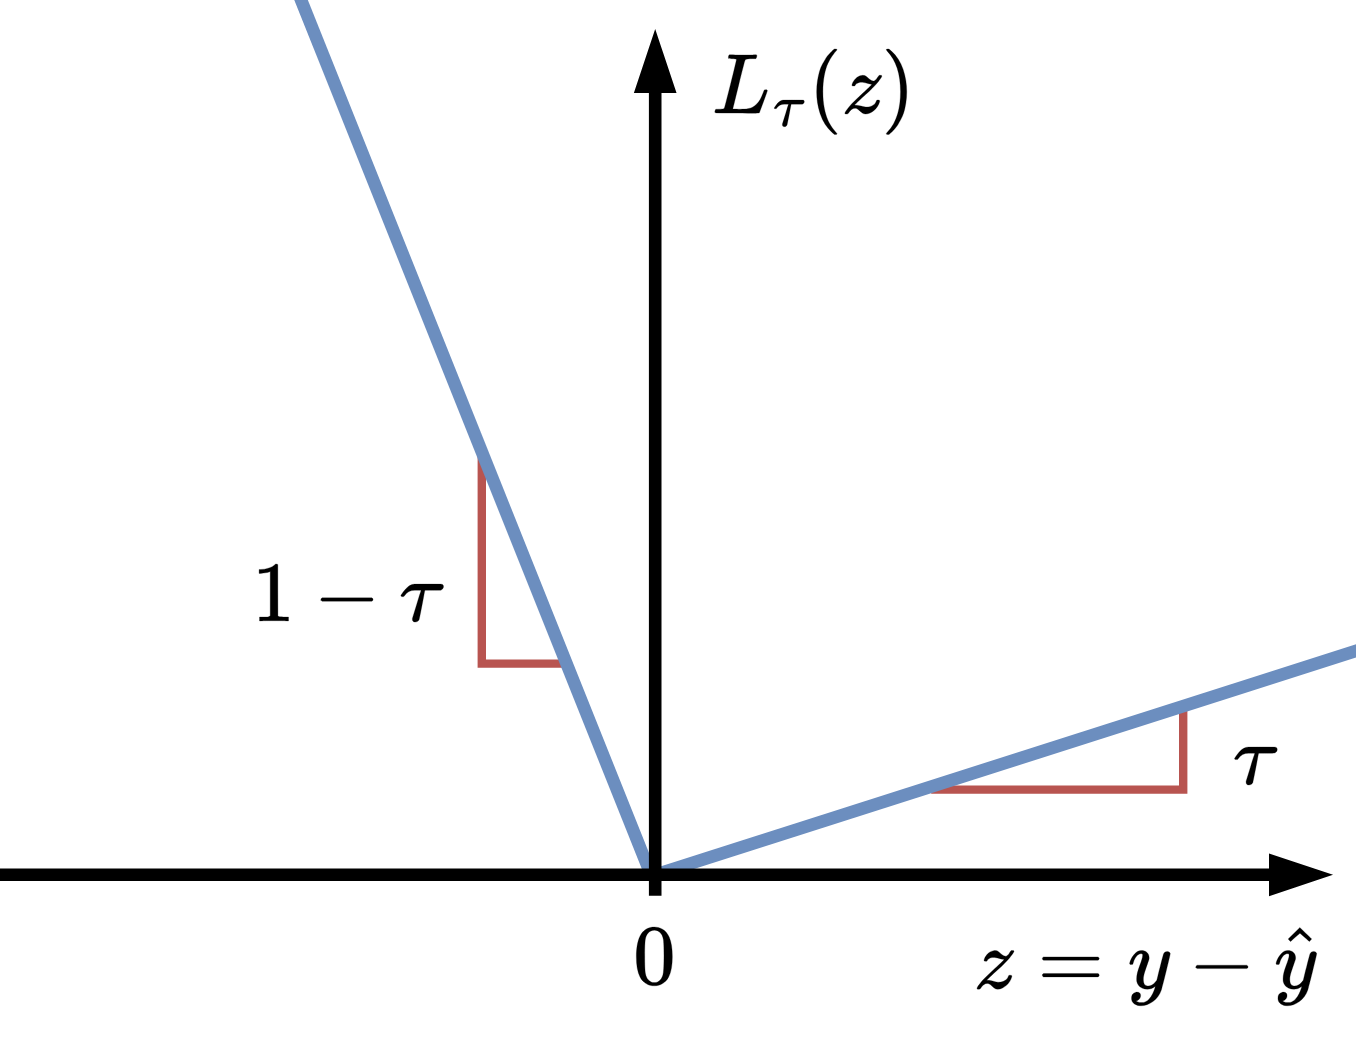
\includegraphics[width=0.5\textwidth]{capitulos/cap_04/imagenes/pinball_loss.png}
        \caption[
            Visualización de la función de pérdida \textit{pinball} para cada valor de error.
        ]{
            Visualización de la función de pérdida \textit{pinball} para cada valor de error.
            Adaptado de la Figura 1 de \cite{romano2019}.
            Esta concretamente muestra la función de pérdida para un cuantil cercano a cero, ya que es más permisivo con los errores positivos que con los negativos, lo cual empujará sus predicciones hacia la parte inferior de la distribución objetivo.
        } 
        \label{fig:pinball_loss}
    \end{figure}

    
    Esta función de pérdida, aplicada a múltiples salidas (cada una asociada a un cuantil específico), busca que las predicciones del modelo cubran la proporción deseada de los datos dentro del intervalo definido por parejas de cuantiles $(\tau_1, \tau_2)$, tratando de cumplir así con un criterio de cobertura probabilística. Por ejemplo: con dos salidas $\tau_1 = 0.05$ y $\tau_2 = 0.95$, se busca que el 90\% las observaciones reales ($y$) estén entre los límites predichos de los dos cuantiles ($\hat{q}_{0.05}$ y $\hat{q}_{0.95}$).

    Además, como ya se comentó al inicio, se puede incluir una tercera salida para el cuantil $\tau_3 = 0.5$, correspondiente a la mediana de la distribución condicional, que actúa como una predicción puntual y es equivalente a minimizar la pérdida \textit{L1}.

    Finalmente, el valor arrojado por la función de pérdida conjunta de los cuantiles se suele expresar como la media de las pérdidas para cada cuantil:
    $$
    \mathcal{L}_{total} = \frac{1}{Q} \sum_{i=1}^Q L_{\tau_i} (y, \hat{q}_{\tau_i})
    $$
    donde $Q$ es el número de cuantiles empleados.

\end{itemize}

Por tanto, este tipo de regresión da una estimación puntual $\hat{y}$ (correspondiente a $\hat{q}_{0.5}$) y una estimación interválica formada por límites inferior y superior $\left[ \hat{q}_{lower}, \hat{q}_{upper} \right]$. Este enfoque es ampliamente aplicable y obtiene intervalos adaptativos a la heterocedasticidad de los datos \cite{romano2019}. Sin embargo, no tiene garantías estadísticas de cobertura bajo distribuciones arbitrarias de errores. Es por ello que se requiere de herramientas adicionales para garantizar la cobertura.

% ------------------------------------------------------------------------------------------------------------

\subsection{Métodos de predicción conformal para regresión}

Todos los métodos propuestos en este trabajo son \textit{split calibration}, es decir, los datos de entrenamiento se dividen en dos subconjuntos: entrenamiento y calibración. No hemos implementado métodos \textit{cross-calibration} como \cite{barber2021} dado que requieren un mayor coste computacional. Además, en los experimentos preliminares, \textit{split calibration} demostró ser suficiente para obtener valores razonablemente buenos de cobertura marginal y una eficiencia adecuada en los intervalos de predicción.

% ------------------------------------------------------------------------------------------------------------

\subsubsection{\textit{Inductive Conformal Prediction} (ICP)}

La \acrshort{ICP} (también conocida como \textit{Split Conformal Prediction}) \cite{papadopoulos2002} fue el primer método de predicción conformal desarrollada para problemas de regresión. Su planteamiento es muy simple: consiste en añadir un margen a las predicciones puntuales, calculado a partir de un cuantil del error absoluto observado en un conjunto de calibración independiente. Este margen permite construir intervalos de predicción que contienen el valor real con una probabilidad determinada previamente (por ejemplo, 90\% o 95\%). 
Por ello, la función de no conformidad es el error absoluto de la predicción respecto al valor real:

$$
NC(x_i, y_i) = | y_i - \hat{f}(x_i) |
% R = \left\{ | y_i - \hat{f}(x_i) | \right\}_{i=1,...,n}
$$

Luego, el umbral de no conformidad para un nivel de confianza $1-\alpha$ se calcula como el cuantil $(1-\alpha)(1+1/n)$ de las puntuaciones de no conformidad:

$$
\delta_\alpha = Quantile_{ \lceil  (1-\alpha) (1 + 1/n)  \rceil } ( \left\{ NC(x_i,y_i) \right\}_{i=1}^n )
$$

Finalmente, para una instancia $x_{n+1}$, el intervalo de predicción $C(x_{n+1})$ se construye como: 

$$
\hat{C_\alpha}(x_{n+1}) = \left[ \hat{f}(x_{n+1}) - \delta_\alpha, \hat{f}(x_{n+1}) + \delta_\alpha\right]
$$

Este método de \acrshort{CP} presenta varias ventajas: 

\begin{itemize}

    \item \textbf{\textit{Model-agnostic}}: Es completamente independiente del modelo y su arquitectura, ya que no utiliza representaciones internas del modelo y solo emplea una salida.  
    
    \item \textbf{Bajo coste computacional}: El método introduce una fase adicional tras el entrenamiento, denominada calibración, en la que se calculan las puntuaciones de no conformidad sobre el conjunto de calibración $\left( O(n_{calib}) \right)$ y se determina el umbral correspondiente mediante el cálculo de cuantiles $\left( O(n_{calib} \log n_{calib}) \right)$. En consecuencia, el coste global es $O(n_{calib} \log n_{calib})$. Aun cuando este orden de complejidad es superior al lineal, en la práctica el tiempo requerido resulta despreciable en comparación con el entrenamiento de modelos complejos, como \textit{ensembles} o \acrshort{DNN}. La inferencia conformal no introduce ningún cambio de orden ($O(1)$), ya que tan solo calcula la puntuación de no conformidad de la nueva instancia para compararla con el umbral. 

\end{itemize}

Sin embargo, también presenta una importante limitación: los \textbf{intervalos generados son simétricos y no adaptativos}, es decir, todos tienen el mismo ancho ($2q_{1-\alpha}$), no permitiéndose adaptarse a la incertidumbre específica de cada predicción.

% \begin{itemize}
    
%     \item \textbf{Intervalo simétrico y no adaptativo}: El intervalo es simétrico, además de tener siempre el mismo ancho ($2q_{1-\alpha}$), no permitiendo adaptarse a la incertidumbre específica de cada predicción. 

%     \item \textbf{Sensibilidad a datos ruidosos o \textit{Out-of-Distribution} (\acrshort{OOD})}: Si el conjunto de calibración contiene \textit{outliers} o viola el supuesto de intercambiabilidad, el umbral \(q_{1-\alpha}\) puede inflarse, generando intervalos excesivamente conservadores. Tampoco detecta heterocedasticidad automáticamente.

% \end{itemize}

% ------------------------------------------------------------------------------------------------------------

\subsubsection{\textit{Conformalized Quantile Regression} (CQR)}

Como su nombre indica, este método se realiza sobre la regresión cuantílica. La \acrshort{CQR} \cite{romano2019} combina la flexibilidad de la regresión cuantílica para estimar directamente los cuantiles condicionales con la garantía de validez estadística proporcionada por la conformalización. Esto permite obtener intervalos de predicción que son asimétricos y adaptativos, ajustándose localmente a la variabilidad y distribución de los datos.

Se ha optado por implementar la segunda definición del intervalo de predicción, presentada en el segundo teorema de \cite{romano2019}, que incluye la calibración de ambas colas para obtener intervalos asimétricos \cite{linusson2014}. Según el artículo, esta opción mejora las garantías de cobertura, aunque puede implicar un aumento en el ancho del intervalo.

El proceso de calibración de este método se lleva a cabo de la siguiente manera: 

\begin{itemize}
    \item Se calculan las puntuaciones de no conformidad sobre los datos del conjunto de calibración como las diferencias entre los valores observados y los límites del intervalo predictivo:
    
    \begin{equation*}
    \begin{split}
        NC_{lower}(x_i,y_i) = \hat{q}_{lower}(x_i) - y_i \\
        NC_{upper}(x_i,y_i) = y_i - \hat{q}_{upper}(x_i)  
    \end{split}
    \end{equation*}

    donde $\hat{q}_{upper}(x_i)$ y $\hat{q}_{lower}(x_i)$ representan los límites superior e inferior del intervalo predictivo para la observación $x_i$, respectivamente, e $y_i$ es el valor observado real.

    \item Se calcula un umbral de no conformidad para un nivel de confianza dado $1-\alpha$ como el cuantil $(1-\alpha)(1+1/n)$ de $R$:

    \begin{equation*}
    \begin{split}
        \delta_{lower_\alpha} &= Quantile_{ \lceil  (1-\alpha) (1 + 1/n)  \rceil } ( \left\{ NC_{lower}(x_i,y_i) \right\}_{i=1}^n  ) \\
        \delta_{upper_\alpha} &= Quantile_{ \lceil  (1-\alpha) (1 + 1/n)  \rceil } ( \left\{ NC_{upper}(x_i,y_i) \right\}_{i=1}^n  )
    \end{split}
    \end{equation*}

\end{itemize}

Tras haber calibrado el modelo, para una instancia $x_{n+1}$, el intervalo de predicción $C(x_{n+1})$ se
construye como:

$$
\hat{C_\alpha}(x_{n+1}) = 
        \left[ 
            \hat{q}_{lower}(x_{n+1}) - \delta_{lower_\alpha}, 
            \hat{q}_{upper}(x_{n+1}) + \delta_{upper_\alpha}
        \right]
$$

En comparación con \acrshort{ICP}:

\begin{itemize}
    \item \acrshort{CQR} no es \textbf{independiente del modelo}, ya que al implementar \acrshort{QR}, requiere de que la arquitectura sea una red neuronal o un modelo \textit{ensemble}. Por tanto, además, requiere de reentrenamiento (a no ser que se partiera de un modelo ya con \acrshort{QR} implementada).
    \item \acrshort{CQR} comparte un \textbf{similar coste computacional}, puesto que realiza prácticamente las mismas operaciones que \acrshort{ICP}, pero para cada límite del intervalo predicho, calibrando los cuantiles inferior y superior de manera independiente para mantener la cobertura deseada. 
    \item \acrshort{CQR} logra \textbf{intervalos asimétricos y adaptativos}, dado que la regresión cuantílica estima directamente los cuantiles condicionales de la distribución de la variable objetivo, permitiendo que los límites del intervalo se ajusten según la heterocedasticidad y la forma local de la distribución de los datos, en lugar de asumir una distribución simétrica o constante del error. 
\end{itemize}

Para cada método se han entrenado 10 modelos independientes desde cero, con el objetivo de capturar la variabilidad inherente al proceso de entrenamiento.

En la Tabla \ref{tab:comparativa_cp} observamos un cuadro comparativo de los distintos métodos presentados para la estimación interválica. 

\renewcommand{\arraystretch}{1.7}
\begin{table}[h]
    \centering
    \begin{tabular}{cccc}
    \toprule
    Característica & ICP & QR & CQR \\ \hline
    %
    Model-agnostic & Sí & Sí & Sí \\
    %
    \begin{tabular}[c]{@{}c@{}}Cobertura marginal\\[-1.2ex]global garantizada\end{tabular} & Sí & No & Sí \\
    %
    \begin{tabular}[c]{@{}c@{}}Cobertura condicional\\[-1.2ex]global garantizada\end{tabular} & No & No & No \\
    %
    % Intervalos asimétricos & No & Sí & Sí \\
    %
    % \begin{tabular}[c]{@{}l@{}}Intervalos \\[-1.1ex] simétricos/asimétricos\end{tabular} & Simétricos & Simétricos & Asimétricos & Asimétricos \\
    %
    Intervalos adaptativos & No & Sí & Sí \\
    %
    Coste calibración   & $O(n \log(n))$    & -- & $O(n \log(n))$ \\
    % 
    \begin{tabular}[c]{@{}l@{}}Coste inferencia \\[-1.2ex] (por predicción)\end{tabular} & $O(1)$ & $O(1)$ & $O(1)$ \\ 
    %
    \bottomrule
    \end{tabular}
    \caption[
        Comparativa de métodos propuestos para problemas de regresión.
    ]{   
        Comparativa de métodos propuestos para problemas de regresión. Las técnicas de \acrshort{CP} son las únicas que garantizan cobertura marginal. Se recuerda que no existe ninguna técnica que garantice la cobertura global condicional.
    }
    \label{tab:comparativa_cp}
\end{table}

% ------------------------------------------------------------------------------------------------------------
% ------------------------------------------------------------------------------------------------------------

\subsection{Calibración de probabilidades en clasificación}

Los modelos de clasificación producen puntuaciones discriminativas, como \textit{logits} o distancias a un hiperplano, pero no siempre reflejan probabilidades reales para la predicción. La \textbf{calibración de probabilidad} en problemas de clasificación en \acrshort{ML} se refiere al ajuste de estas puntuaciones de salida para que reflejen más fielmente probabilidades de predicción. 

La calibración de probabilidades busca que cuando un modelo diga ``X\% de probabilidad'', eso corresponda de verdad a la frecuencia observada en los datos. Por ejemplo, si un modelo asigna una probabilidad del 70\% a un conjunto de instancias, aproximadamente 7 de cada 10 deberían pertenecer a la clase positiva si el modelo está bien calibrado.

Existen distintas técnicas de post-procesamiento para mejorar la calibración. En este trabajo se empleará \textbf{Temperature Scaling} \cite{guo2017}, algoritmo usado principalmente en redes neuronales profundas. Este ajusta los \textit{logits} dividiéndolos por un parámetro de temperatura $T>0$, de manera que:
\begin{itemize}
    \item Si $T>1$, las puntuaciones se suavizan, disminuyendo la confianza excesiva del modelo.
    \item Si $T<1$, las puntuaciones se vuelven más extremas, aumentando la confianza.
\end{itemize}
El parámetro $T$ se aprende sobre un conjunto de validación independiente, optimizando la entropía cruzada de las predicciones ajustadas con respecto a las etiquetas reales. De esta manera, se mejora la calibración sin afectar la discriminación del modelo, es decir, las clases más probables siguen siendo las mismas.

Entre sus ventajas destacan:
\begin{itemize}
    \item Muy simple: un solo parámetro.
    \item Mantiene la discriminación de las clases.
    \item Efectivo para corregir sobreconfianza típica en redes profundas.
\end{itemize}

Se ha escogido este algoritmo ya que es el utilizado en trabajos recientes sobre técnicas de Conformal Prediction para clasificación \cite{angelopoulos2020, huang2023conformal}.

% ------------------------------------------------------------------------------------------------------------
% ------------------------------------------------------------------------------------------------------------

\subsection{Métodos de predicción conformal para clasificación}

\subsubsection{Least-Ambiguous set-valued Classifiers (LAC)}

\acrshort{LAC} \cite{sadinle2019} es el primer método propuesto de predicción conformal para problemas de clasificación. Propone un enfoque de clasificación de conjuntos de valores (\textit{set-valued classification}) en el que, en lugar de asignar una única etiqueta a cada instancia, se selecciona un conjunto de etiquetas que garanticen un nivel de confianza predeterminada por el usuario.

La función de no conformidad es conocida como \textbf{probabilidad inversa o \textit{hinge loss}} \cite{johansson2017}, y se calcula como la unidad menos la probabilidad de la clase verdadera%
\footnote{
    Se le denomina probabilidad a un valor de certeza que realmente no tiene garantías estadísticas, ya que proviene directamente de la salida \textit{softmax} o sigmoide del modelo. Estas salidas no están necesariamente bien calibradas ni corresponden a verdaderas probabilidades, si bien el término se utiliza frecuentemente por motivos de simplicidad y comunicación.
}
o, lo que es lo mismo, la suma de valores de probabilidad de todas las clases salvo la correspondiente a la etiqueta verdadera:
$$
NC(x_i,y_i) = 1- \hat{\pi}_{y_i}(x_i)
$$

donde $\hat{\pi}_{y_i}(x_i)$ es la probabilidad para la clase de la etiqueta verdadera%
\footnote{
    $\hat{\pi}(x_i)$ es el vector de probabilidades de las clases para la instancia $i$.
}.


El umbral de no conformidad para un nivel de confianza $1-\alpha$ se calcula como el cuantil 
$(1-\alpha)(1+1/n)$ de las puntuaciones de no conformidad:

$$
\delta_\alpha = Quantile_{ \lceil  (1-\alpha) (1 + 1/n)  \rceil } ( \left\{ NC(x_i,y_i) \right\}_{i=1}^n)
$$

El conjunto de predicción conformal de una nueva instancia $x_{n+1}$ se construye como las clases cuyas probabilidades superan la unidad menos el umbral de no conformidad (véase la Figura \ref{fig:LAC_threshold}):

$$
\Gamma_\alpha(x_{n+1}) = \left\{ k | \hat{\pi}_k(x_{n+1}) \ge 1-\delta_\alpha \right\} 
$$

\begin{figure}[h]
    \centering
    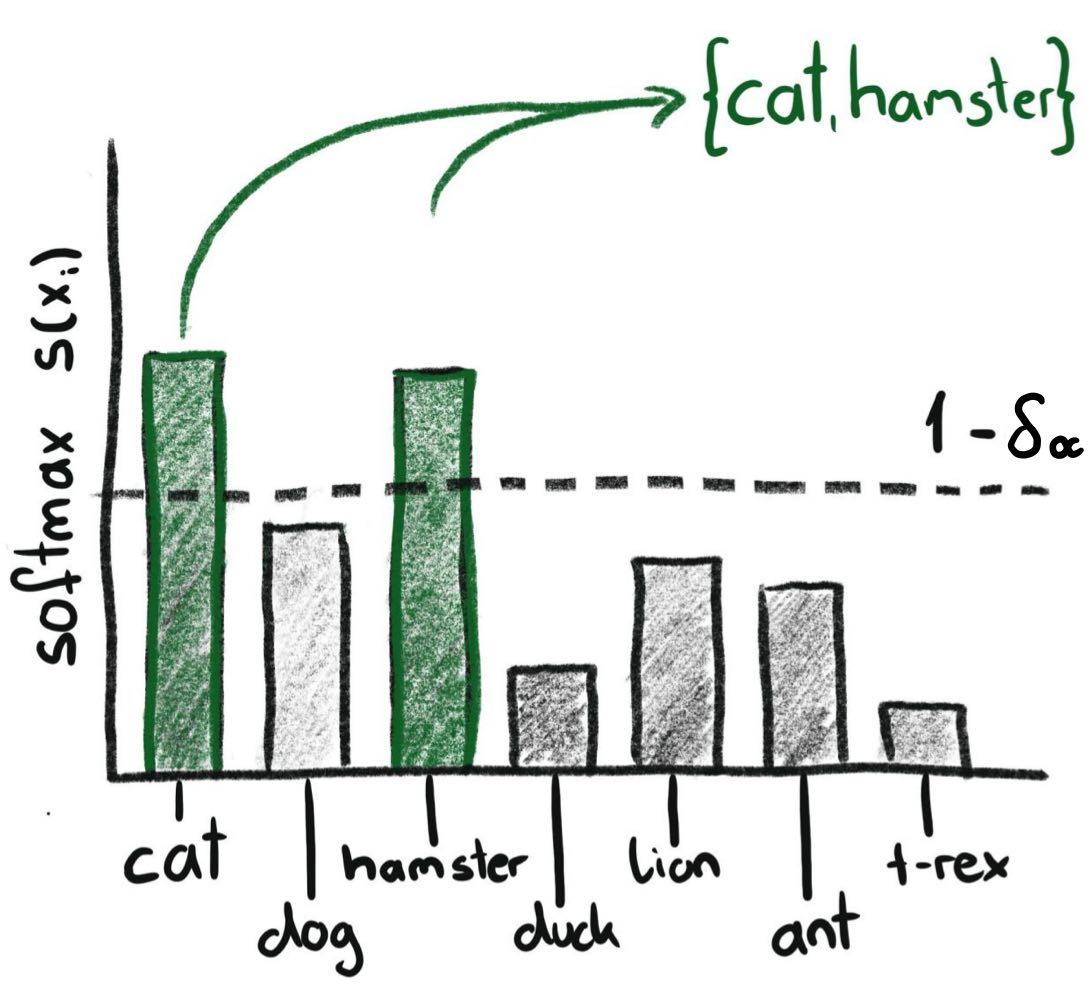
\includegraphics[width=0.6\textwidth]{capitulos/cap_04/imagenes/LAC_threshold.jpg}
    \caption[
        Ejemplo de selección de clases para el conjunto conformal en LAC. 
    ]{
        Ejemplo de selección de clases para el conjunto conformal en \acrshort{LAC}. Se escogen aquellas clases que presentan una puntuación \textit{softmax} mayor a $1-\delta_\alpha$. Adaptado de \cite{mindfulmodeler2023week1}.
    }
    \label{fig:LAC_threshold}
\end{figure}

Así, se seleccionan aquellas clases cuya probabilidad es lo suficientemente alta como para superar el umbral de no conformidad previamente calculado. No obstante, puede ocurrir que, para ciertas instancias, ninguna clase alcance dicho umbral, lo que resultaría en un conjunto de predicción vacío. Para evitar esta situación, se ha optado por incluir en estos casos todas las clases posibles dentro del conjunto de predicción. Esta elección responde a una estrategia conservadora: ante la falta de evidencia suficiente para respaldar alguna clase en particular con el nivel de confianza requerido, lo más prudente es no excluir ninguna posibilidad, y así reflejar una alta incertidumbre. 

Algunas propiedades de este método son:

\begin{itemize}

    \item \textbf{\textit{Model agnostic}}: Es independiente del modelo, ya que solo necesita el vector de puntuaciones predictivas $\hat{\pi}(x_i)$ y la etiqueta verdadera para cada instancia $y_i$.  

    \item \textbf{Conjuntos de predicción no adaptativos}: A pesar de poder presentar conjuntos con distinto número de clases predichas, 
    
    
    emplea un único umbral calibrado globalmente sobre todas las muestras y clases por igual. Este enfoque no ajusta dinámicamente el tamaño del conjunto de predicción en función de la incertidumbre del modelo para cada instancia.

    \item \textbf{Bajo coste computacional}: Al igual que pasaba en regresión, solo añade coste computacional en la calibración, con el cálculo de puntuaciones de no conformidad ($O(n_{calib})$) y la obtención del umbral de no conformidad ($O(n_{calib} \textnormal{log } n_{calib})$). No añade coste a la inferencia ($O(1)$).
    
\end{itemize}

% ------------------------------------------------------------------------------------------------------------

\subsubsection{Mondrian Confidence Machine (MCM)}

\acrshort{MCM} \cite{vovk2003} es un método estrechamente relacionado con \acrshort{LAC}, ya que emplea el mismo esquema general de \acrshort{CP}. Sin embargo, introduce una diferencia clave: en lugar de aplicar un único umbral global para todas las clases, \acrshort{MCM} segmenta el conjunto de calibración por clase y calcula las puntuaciones y los umbrales de no conformidad de forma independiente para cada una (véase la Figura \ref{fig:mondrian_diagram}).

\begin{figure}[h]
    \centering
    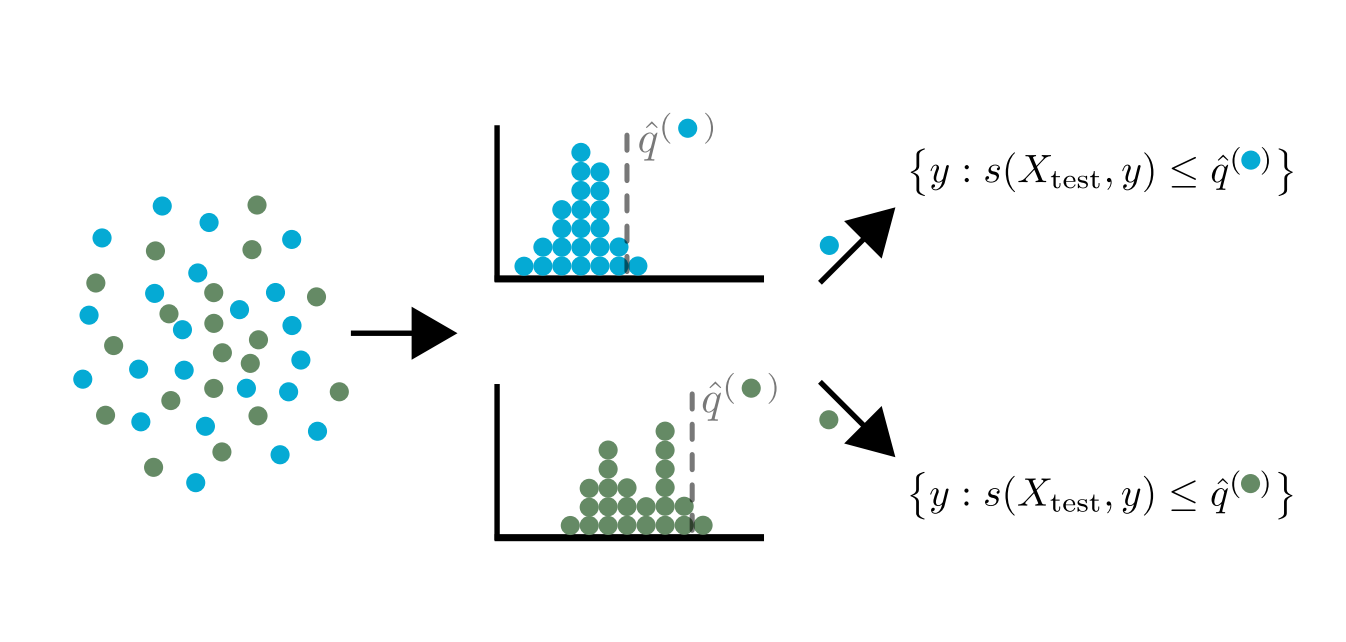
\includegraphics[width=0.9\textwidth]{capitulos/cap_04/imagenes/mondrian_diagram.png}
    \caption[
        Diagrama ilustrativo de la división de ejemplos utilizada en MCM.
    ]{
        Diagrama ilustrativo de la división de ejemplos utilizada en \acrshort{MCM}. Para cada clase se calcula un umbral de no conformidad a partir de las puntuaciones de no conformidad de los ejemplos pertenecientes a esa clase.
    }
    \label{fig:mondrian_diagram}
\end{figure}

A continuación, se detallan sus principales característica diferenciadas de \acrshort{LAC}:

\begin{itemize}

    \item \textbf{Garantiza cobertura condicional por clase}, lo cual es muy útil en conjuntos desbalanceados. A diferencia de \acrshort{APS}, que ofrece cobertura marginal sobre el conjunto total, MCM busca asegurar que cada clase individual cumpla el nivel de cobertura deseado, lo que favorece una distribución más equitativa del error.

    \item \textbf{Coste computacional comparable a \acrshort{LAC}}: Al igual que LAC, MCM calcula las puntuaciones de no conformidad para todas las instancias del conjunto de calibración. Posteriormente, para cada clase se ordenan las puntuaciones de su subconjunto para determinar el umbral correspondiente. Si hay $K$ clases y $n_k$ instancias por clase, el coste total de esta fase es $\sum_{k=1}^{K} O(n_k \log n_k)$, que en la práctica se aproxima a $O(n_{calib} \log n_{calib})$, manteniendo la complejidad algorítmica de LAC. En la fase de inferencia, la predicción para una nueva instancia requiere únicamente calcular la puntuación de no conformidad y compararla con el umbral de su clase, lo que supone un coste lineal respecto al número de clases, $O(K)$, que se sigue traduciendo en tiempos prácticamente despreciables para la inmensa mayoría de problemas. Por tanto, MCM sigue siendo eficiente.

\end{itemize}

% ------------------------------------------------------------------------------------------------------------

\subsubsection{Adaptive Prediction Sets (APS)}

\acrshort{APS} \cite{romano2020}, como sugiere su nombre, tiene como objetivo generar conjuntos de predicción adaptativos, cuyo tamaño se ajusta dinámicamente en función de la incertidumbre del modelo para cada muestra. De este modo, se busca que las predicciones sean más informativas y reflejen con mayor precisión la confianza del modelo.

La función de no conformidad utilizada en \acrshort{APS} evalúa, para cada instancia, la probabilidad total acumulada en aquellas clases que el modelo considera al menos tan probables como la clase verdadera. En otras palabras, se calcula como la suma de las probabilidades predichas para todas las clases cuya probabilidad es mayor o igual a la asignada a la etiqueta correcta.

Sea el vector $\hat{\pi}$ ordenado en orden decreciente: 
$$
\hat{\pi}_{(1)}(x_i) \ge \hat{\pi}_{(2)}(x_i) \ge \cdot\cdot\cdot \ge \hat{\pi}_{(K)}(x)
$$
donde $(k)$ es el índice de la clase con la $k$ mayor probabilidad, la función de no conformidad se define como:
$$
NC(x_i, y_i) = \sum_{j=1}^k \hat{\pi}_{(j)}(x_i) \textnormal{ donde } (k)=y_i 
$$

Cabe destacar que, en el caso particular de clasificación binaria, esta medida de no conformidad coincide exactamente con la utilizada en el método \acrshort{LAC}, ya que la acumulación se limita a una o dos clases. Por tanto, ambos métodos resultan equivalentes en este escenario. Sin embargo, divergen en problemas multiclase, donde las puntuaciones de no conformidad de \acrshort{APS} son más permisivas que las de \acrshort{LAC}, ya que reconocen que un modelo puede identificar características comunes entre varias clases y generar valores probabilísticos repartidos. No existe incertidumbre cuando la puntuación probabilística más alta corresponde a la clase verdadera. Por tanto, \acrshort{APS} penaliza menos los casos en que la clase correcta está entre las más probables, aunque no necesariamente en primer lugar.

A partir de las puntuaciones de no conformidad en el conjunto de calibración, se calcula el umbral de no conformidad de la manera habitual:

$$
\delta_\alpha = Quantile_{ \lceil  (1-\alpha) (1 + 1/n)  \rceil } ( \left\{ NC(x_i,y_i) \right\}_{i=1}^n )
$$

Tras la calibración, para una nueva instancia $x_{n+1}$, se calcula la distribución de probabilidad ordenada en orden decreciente, y se suman de forma acumulada las probabilidades desde la clase más probable hasta que dicha suma sea mayor o igual que el umbral calibrado. El conjunto de predicción $\Gamma_\alpha(x_{n+1})$ se forma entonces incluye todas las clases correspondientes a ese conjunto acumulado: 

$$
\Gamma_\alpha(x_{n+1}) = \left\{ (1),...,(k) \right\} \\ \textnormal{ donde } 
k = min\left\{ j: \sum_{i=1}^{j} \hat{\pi}_{(i)}(x_{n+1}) \ge \delta_\alpha \right\} 
$$


\paragraph{Componente aleatoria}

Una extensión útil de \acrshort{APS} consiste en introducir una componente aleatoria durante la fase de calibración para compensar la tendencia del método a la \textit{sobrecobertura}. En este ajuste, cuando se calcula la puntuación de no conformidad para una instancia de calibración, se decide excluir la contribución de la última clase incluida (aquella correspondiente a la etiqueta verdadera $y_i$) con una probabilidad proporcional al exceso de cobertura ---respecto al nivel de confianza $1-\alpha$--- que dicha clase genera.

Formalmente, sea:
$$
V_i = \frac{NC(x_i, y_i) - (1-\alpha)}{\hat{\pi}_{(k)}(x_i)} \quad \text{con} \quad (k) = y_i
$$
donde $A$ es la puntuación de no conformidad estándar de \acrshort{APS} y $\hat{\pi}_{(k)}$ la probabilidad de la última clase incluida. Se genera un valor aleatorio $u_i \sim \mathcal{U}(0,1)$ y, si $u_i > V_i$ y la clase verdadera no está en primera posición ($k \ge 2$), se elimina completamente la contribución de dicha clase de la suma acumulada. En caso contrario, se mantiene la puntuación original.

De este modo, las instancias en las que la última clase aporta un exceso notable de cobertura tienen mayor probabilidad de ser recortadas, reduciendo así el umbral de no conformidad $\delta_\alpha$ y produciendo conjuntos de predicción más pequeños, sin comprometer significativamente la cobertura global. En la fase de inferencia, el procedimiento de construcción de $\Gamma_\alpha(x_{n+1})$ se mantiene idéntico, pero el umbral reducido provoca que se necesiten menos clases para alcanzar el criterio, generando así \textbf{conjuntos de predicción más pequeños} en promedio, y que siguen garantizando estadísticamente la cobertura marginal.

Las principales características de APS son las siguientes:

\begin{itemize}
    \item Este algoritmo solo garantiza cobertura marginal, pero genera \textbf{conjuntos de predicción más adaptativos} respecto a la incertidumbre inherente a la predicción de cada instancia. A diferencia de métodos con umbrales fijos, ajusta dinámicamente el tamaño de los conjuntos según la confianza del modelo en regiones específicas del espacio de características.
    
    Sin embargo, en la práctica se ha observado que esta adaptabilidad conlleva \textbf{conjuntos de predicción más grandes en promedio que los de LAC} \cite{romano2020, angelopoulos2020}. Este fenómeno es un \textit{trade-off} inherente al intentar aproximar la cobertura condicional sin asumir distribuciones subyacentes.
    
    \item El \textbf{coste computacional resulta más elevado que los dos algoritmos previos}. Durante la fase de calibración, cada ejemplo requiere ordenar las probabilidades de las clases para calcular su puntuación de no conformidad, lo que implica un coste total de $O(n_{calib} \cdot K \log K)$ donde $K$ es el número total de clases. En la fase de inferencia, el procedimiento se repite para cada nueva instancia: se ordenan las clases por probabilidad y se van acumulando hasta superar el cuantil de calibración, alcanzando un coste de $O(K \log K)$ por predicción. Aunque este orden es superior al del método clásico, en la práctica sigue siendo asumible para valores moderados de $K$.
    
\end{itemize}

% ------------------------------------------------------------------------------------------------------------

\subsubsection{Regularized Adaptive Prediction Sets (RAPS)}

\acrshort{RAPS} \cite{angelopoulos2020} es una variante del método APS, que introduce modificaciones clave para reducir el tamaño de los conjuntos de predicción, especialmente en escenarios con muchas clases, donde \acrshort{APS} tiende a generar conjuntos excesivamente grandes. El objetivo principal de \acrshort{RAPS} es mantener la propiedad de cobertura marginal deseada, al tiempo que se obtienen conjuntos de predicción más compactos y útiles en la práctica. 

\acrshort{RAPS} extiende la función de no conformidad utilizada en \acrshort{APS} mediante la incorporación de un término de regularización que penaliza explícitamente la inclusión de clases con baja probabilidad en conjuntos de predicciones de tamaño ya elevado. 

Para ello, se introducen dos hiperparámetros en la función de no conformidad:

\begin{itemize}

    \item $k_{reg}$ representa el tamaño mínimo del conjunto de predicción a partir del cual se comenzará a aplicar penalización. Es decir, los conjuntos de predicción de tamaño menor o igual a $k_{reg}$ no serán penalizados, ya que se asume que, si todos los conjuntos tuvieran como máximo ese tamaño, la cobertura marginal aún se mantendría. 
    
    El valor de este hiperparámetro se determina empíricamente observando, en el conjunto de calibración, cuál es el menor tamaño de conjunto que cumple con la cobertura deseada en una fracción suficientemente alta de las instancias. 
   
    \item $\lambda$, un parámetro de regularización que penalizará más a aquellos conjuntos que superen $k_{reg}$ etiquetas predichas cuanto mayor número de etiquetas tengan. 

    Este hiperparámetro se determina típicamente a través de validación en un conjunto de datos independiente al de calibración, mediante búsqueda de hiperparámetros que minimicen el tamaño medio del conjunto de predicción sin comprometer significativamente la cobertura marginal. En la práctica, se suele probar con varios valores posibles para $\lambda$ y seleccionar el que logre el mejor equilibrio entre concisión y cobertura en el conjunto de validación.

\end{itemize}

Una vez determinados los valores de estos hiperparámetros, se calculan las puntuaciones de no conformidad de la siguiente manera:

$$
NC(x_i, y_i) = \sum_{j=1}^k \hat{\pi}_{(j)}(x_i) + \lambda (k-k_{reg})^+ \textnormal{ donde } (k) = y_i
$$

El procedimiento de calibración y predicción en \acrshort{RAPS} sigue la misma estructura general que \acrshort{APS}, pero utiliza la función de no conformidad regularizada en lugar de la acumulación pura de probabilidades. Así, el umbral calibrado se calcula como:

$$
\delta_\alpha = Quantile_{ \lceil  (1-\alpha) (1 + 1/n)  \rceil } \left( \left\{ NC(x_i,y_i) \right\}_{i=1}^n \right)
$$

Y el conjunto de predicción para una nueva instancia $x_{n+1}$ se construye como

\begin{align*} 
\Gamma_\alpha(x_{n+1})= &\left\{ (1), ..., (k) \right\} \textnormal{ donde }\\
& k = \min \left\{ j: \sum_{i=1}^{j} \pi_{(i)}(x_{n+1}) + \lambda (k-k_{reg})^+  \ge \delta_\alpha \right\}
\end{align*}

Gracias a la regularización, \acrshort{RAPS} tiende a generar \textbf{conjuntos de predicción más pequeños que \acrshort{APS}}, especialmente cuando la clase verdadera se encuentra entre las más probables (y por tanto el hiperparámetro $k_{reg}$ tiene un valor bajo).

Al igual que \acrshort{APS}, también admite una \textbf{componente aleatoria}, que funciona de igual manera: durante la fase de calibración, se calcula para cada instancia la probabilidad de excluir la contribución de la última clase incluida ---aquella correspondiente a la etiqueta verdadera--- considerando también el término de regularización, en función del exceso de cobertura que produce respecto al nivel nominal $1-\alpha$.

Al tratarse de una extensión de \acrshort{APS}, \acrshort{RAPS} tiene un \textbf{orden algorítmico idéntico a \acrshort{APS}}, aunque en la práctica \acrshort{RAPS} puede ser ligeramente más costoso debido al paso extra de regularización. 

% ------------------------------------------------------------------------------------------------------------

\subsubsection{Sorted Adaptive Prediction Sets (SAPS)}

\acrshort{SAPS} \cite{huang2023conformal} propone un enfoque distinto a métodos previos como \acrshort{APS} y \acrshort{RAPS}. Los autores identifican una limitación importante en estos algoritmos: las probabilidades producidas por la capa \textit{softmax} suelen seguir una distribución con cola larga, lo que facilita la inclusión de clases poco probables en los conjuntos de predicción. Esto lleva a la generación de conjuntos innecesariamente grandes, que reducen la utilidad práctica del método.

\acrshort{SAPS} argumenta que muchas de estas probabilidades de baja magnitud representan información redundante o poco útil para la tarea de predicción conforme. En lugar de utilizar todo el vector de probabilidades, propone construir los conjuntos de predicción únicamente a partir de dos elementos clave: 
\begin{itemize}
    \item la probabilidad más alta (asociada a la clase predicha como más probable), y
    \item el orden de clasificación de las clases según el modelo.
\end{itemize}

A partir de esta representación reducida, las clases se ordenan por probabilidad decreciente y se define una función de no conformidad que combina la probabilidad máxima con la posición $k$ de la clase verdadera en el ranking. El objetivo es que la inclusión de una clase dependa más de su relevancia relativa que de su probabilidad absoluta, evitando el efecto adverso de las colas largas.

A diferencia de los anteriores métodos adaptativos, este método incluye la \textbf{componente aleatoria} desde su planteamiento inicial. La función de no conformidad propuesta es:

$$
NC(x_i, y_i) = \hat{\pi}_{max}(x_i) + \lambda \,(k - 2 + u_i)
$$

donde:  
\begin{itemize}
    \item $\hat{\pi}_{\max}(x_i)$ corresponde a la probabilidad más alta predicha por el modelo,  
    \item $\lambda$ es un parámetro de regularización que incrementa la penalización a medida que la clase verdadera se aleja de las primeras posiciones del ranking,  
    \item $k$ indica la posición de $y_i$ en el ranking de salida (con $k=1$ para la clase más probable, $k=2$ para la segunda, y así sucesivamente),  
    \item $u_i \sim \mathcal{U}(0,1)$ introduce un componente aleatorio continuo que suaviza la penalización y evita empates exactos.
\end{itemize}

Observe que la penalización efectiva se aplica sobre el término $k - 2 + u_i$: no se penaliza la clase en primera posición ($k=1$), mientras que para las siguientes posiciones la penalización crece de forma lineal. La inclusión de $u_i$ hace que la penalización de la última clase considerada se distribuya de manera uniforme en el intervalo $(k-1, k)$, lo que garantiza aleatoriedad controlada y una calibración más estable.

El umbral de no conformidad $\delta_\alpha$ se calcula a partir de las puntuaciones $NC(x_i, y_i)$ en el conjunto de calibración, de forma análoga a \acrshort{APS} y \acrshort{RAPS}:
$$
\delta_\alpha = Quantile_{\lceil (1-\alpha)(1+1/n) \rceil} \left( \left\{ NC(x_i, y_i) \right\}_{i=1}^n \right)
$$

En la fase de inferencia, el conjunto de predicción para una nueva instancia $x_{n+1}$ se construye añadiendo las clases en orden decreciente de probabilidad, calculando para cada una la puntuación de no conformidad y deteniéndose cuando esta supera el umbral $\delta_\alpha$:

\begin{align*}
\Gamma_\alpha(x_{n+1}) = &\left\{ (1), \dots, (k) \right\} \ \textnormal{donde} \\
& k = \min \left\{ j : \hat{\pi}_{max}(x_{n+1}) + \lambda (j - 1) \ge \delta_\alpha \right\}
\end{align*}

Gracias a esta estrategia basada en orden y probabilidad máxima, \acrshort{SAPS} intenta generar conjuntos de predicción más compactos que \acrshort{APS} y \acrshort{RAPS} en escenarios con distribuciones de salida muy sesgadas, manteniendo la cobertura marginal deseada y reduciendo la inclusión de clases irrelevantes.

El \textbf{coste computacional es idéntico al de \acrshort{APS}} tanto en orden algorítmico como en las operaciones realizadas con las implementaciones realizadas para este trabajo.


En la Tabla \ref{tab:comparativa_cp_classification} observamos un cuadro comparativo de los distintos métodos presentados para la estimación de conjuntos predictivos. 

\renewcommand{\arraystretch}{1.8}
\begin{table}[h]
    \centering
    \begin{tabular}{cccc}
    \toprule
    Característica & LAC & MCM & (R/S)APS \\ \hline
    %
    Model-agnostic & Sí & Sí & Sí \\
    %
    \begin{tabular}[c]{@{}c@{}}Cobertura marginal\\[-1.4ex]global garantizada\end{tabular} & Sí & Sí & Sí \\
    %
    \begin{tabular}[c]{@{}c@{}}Cobertura condicional\\[-1.4ex]por clase garantizada\end{tabular} & No & Sí & No \\
    %
   \begin{tabular}[c]{@{}l@{}}Conjuntos de\\[-1.4ex]tamaño variable\end{tabular} & Sí & Sí & Sí \\
    %
    Conjuntos adaptativos & No & No & Sí \\
    %
    Coste calibración   & $O(n \log(n))$    & $O(n \log(n))$ & $O(n K \log(K))$ \\
    % 
    \begin{tabular}[c]{@{}l@{}}Coste inferencia \\[-1.4ex] (por predicción)\end{tabular} & $O(1)$ & $O(1)$ & $O(K \log(K))$ \\ 
    %
    \bottomrule
    \end{tabular}
    \caption[
        Comparativa de métodos propuestos para problemas de clasificación.
    ]{   
        Comparativa de métodos propuestos para problemas de clasificación. 
    }
    \label{tab:comparativa_cp_classification}
\end{table}

% ------------------------------------------------------------------------------------------------------------
% ------------------------------------------------------------------------------------------------------------
